\def\code#1{\texttt{#1}}
\lstset{language=Python}  

\section{Coding Style}
\label{sec:cs}

Hier einige Leitlinien für einen sauberen und auch von anderen gut lesbaren Python-Code.

\begin{itemize}
	\item Grundsätzlich orientieren wir uns an \href{http://legacy.python.org/dev/peps/pep-0008/#introduction}{PEP8}, einem der am weitesten verbreiteten Standards für Python-Code. Die Quintessenz davon ist:
	\begin{itemize}
		\item \code{import}-Statements sollten sich am Anfang der Datei befinden, es sollte nur importiert werden, was auch wirklich gebraucht wird.

		\item Operatoren sind sinnvoll mit Whitespace zu umgeben:
		\lstinputlisting{resources/ws.py}

		\item Sinnvolles setzten von neuen Zeilen: logisch getrennte Blöcke innerhalb einer Funktion/Aufgabe mit einer, Aufgaben, Klassen, etc. mit zwei neuen Zeilen voneinander trennen.

		\item Am einfachsten lässt sich das mit einem guten Plugin einhalten; für Atom gibt es \emph{atom-beautify}, das einen den Großteil der Arbeit abnimmt.
	\end{itemize}

	\item Sprechender Code ist besser als Kommentare! Es ist einfacher und schneller (für den Leser des Codes) den Sinn von einigen Zeilen Code zu erkennen, wenn dieser gut benannte Variablen, Funktionen, etc. besitzt. Kommentare sind sparsam zu verwenden und kurz zu halten; nur wenn sich die Funktionsweise/der Sinn nicht aus dem Code ergibt oder eine Zeile nicht ersichtliche 'Nebenwirkungen' hat, ist ein Kommentar angebracht.

	\item Wenn möglich \emph{docstrings} verwenden statt Kommentaren! Zum Beispiel kann man eine Methode so kommentieren:
	\lstinputlisting{resources/meth.py}
	Der Vorteil liegt darin, dass ein 'Kommentar' in dieser Form dann immer erscheint, wenn man diese Methode aufruft (wenn man seinen Texteditor richtig eingestellt hat, duh).

	\begin{figure}[H]
		\centering
		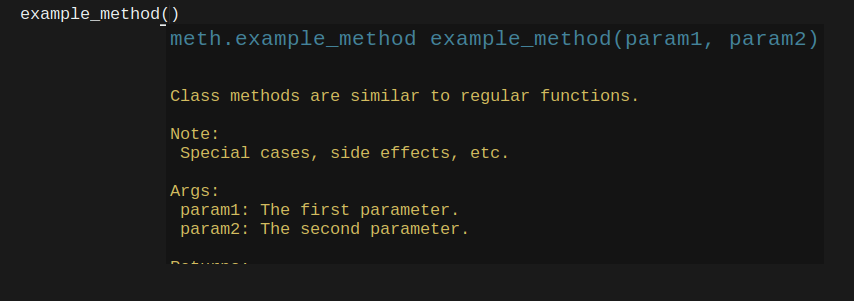
\includegraphics[width=10cm,height=7cm,keepaspectratio]{resources/helper.png}
	\end{figure}

	Insbesondere die Datentypen, die die Methode annimmt und ausgibt sollten spezifiziert werden, wenn dies nicht aus der Benennung hervorgeht (\code{IsWindowOpen()} gibt mit Sicherheit ein boolean zurück, bei \code{GenerateInfoGraphic()} ist das aber nicht mehr klar). Docstrings können auch für Variablen genutzt werden.

	\item Ein für Physiker sinnvolle naming convention ist folgende:
	\begin{itemize}
		\item Variablennamen und Funktionen benutzen Kleinschreibung für Wörter, physikalische Bezeichner (\code{T} für Temperatur, \code{phi} für einen Winkel) werden so gut es geht in gültige Variablennamen übertragen.

		\item Zum Trennen von Wörtern sind Unterstriche zu verwenden.

		\item Meistens ist anders als in einer Rechnung auf Papier nicht sofort ersichtlich, was für ein Winkel, etc. gemeint ist; es schadet selten, einen Variablennamen zu wählen, der auch noch 15 Zeilen später aussagekräftig ist.

		\item Hilfsvariablen sind sinnvoll zu benennen; \code{m2} und \code{bla} sind sehr schlechte Namen für Variablen, auch wenn man sie nur für ein paar Zeilen braucht. Es erleichtert das Lesen des Codes ungemein, diesen aussagekräftige Namen zu geben. Nebenbei findet man so auch Fehler im eigenen Code schneller.\\
		Einen einfachen counter in einer for-Schleife, dessen Sinn auch ohne langen Namen ersichtlich ist, muss man aber nicht umändern.

		\item Wenn eine Variable einheitenbehaftet ist, wird die Einheit hinter der Deklaration angegeben. Es sind immer Grundeinheiten zu verwenden (also etwa immer Meter, nie Kilometer).

		\item Beispiel:
		\lstinputlisting{resources/naming.py}
	\end{itemize}

\end{itemize}

Diese Leitlinien sind nur ein erster Vorschlag; bitte übt Kritik! Ein solcher Standard hilft enorm, aber wir müssen ihn alle als akzeptabel befinden, damit ihn auch jeder gerne nutzt.